
\subsection{Dirichlet Process}

The Dirichlet process is a stochastic process used in Bayesian non-parametric models. Each draw from a Dirichlet process is itself a discrete distribution. For a random distribution $G$ to be distributed according to a DP, its marginal distributions have to be Dirichlet distributed. Let $H$ bea distribution over $\Theta$ and $\alpha$ be a positive real number. We say that $G$ is a Dirichlet process distributed with \textit{base distribution} $H$ and \textit{concentration parameter} $\alpha$ if:

\begin{equation}
    (G(A_1),...,G(A_r)) \sim \mathrm{Dir}(\alpha H(A_1),...,\alpha H(A_r))
\end{equation}
for every finite measurable partition $A_1$,...,$A_r$ of $\Theta$, where Dirichlet distribution is defined as:
\begin{equation}
    p(x_1,...,x_K) = \frac{\Gamma(\sum_k \alpha_k)}{\prod_k \Gamma(\alpha_k)}\prod_{k=1}^{K}x_{k}^{\alpha_k-1}
\end{equation}
The base distribution is the mean of the DP: $E[G(A)] = H(A)$, whereas the concentration parameteris the inverse variance: $V[G(A)] = H(A)(1-H(A))/(\alpha+1)$ for any measureable set $A\subset \Theta$. The larger the $\alpha$, the smaller the variance, and the DP will concentrate more of its mass around the mean.
\begin{figure}[tbhp]
    \centering
    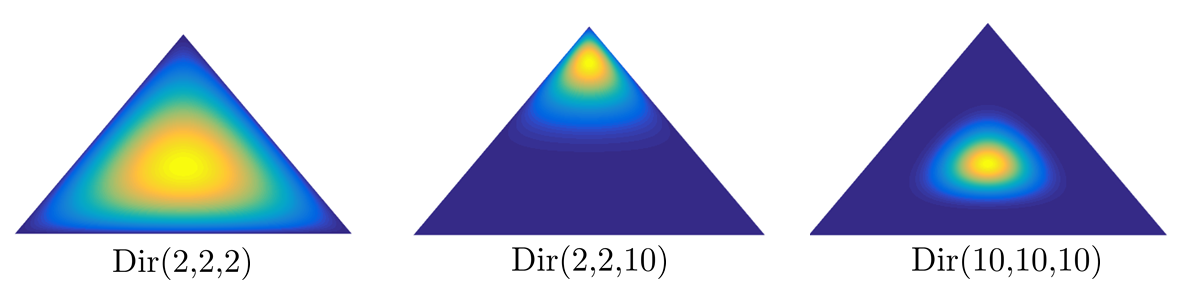
\includegraphics[width=0.8\textwidth, trim={10 10 10 10}]{figures/dir_merged.png}
    \caption{Dirichlet distribution: $\mathrm{Dir}(\alpha_1,\alpha_2,\alpha_3)$ over the simplex.}
    \label{fig:dir_merged}
\end{figure}
Let $\theta_1,...,\theta_n$ be a sequence of independent draws from $G\sim DP(\alpha,H)$. We are interested in the posterior distribution of G given observed values of $\theta_1,...,\theta_n$. Let $n_k$ be the number of observed values in $A_k$, the by conjugacy the Dirichlet and multinomial distributions we have:
\begin{equation}
    (G(A_1),...,G(A_r))|\theta_1,...,\theta_n \sim \mathrm{Dir}(\alpha H(A_1)+n_1,...,\alpha H(A_r)+n_r)
\end{equation}
The posterior is also a DP with an updated concentration parameter and base distribution:
\begin{equation}
    G|\theta_1,...,\theta_n \sim DP(\alpha+n, \frac{\alpha}{\alpha+n}H + \frac{n}{\alpha+n}\frac{\sum_{i=1}^{N}\delta_{\theta_i}}{n})
\end{equation}
Note that the posterior base distribution is a weighted average between the prior base distribution $H$ and the empirical distribution $\frac{1}{n}\sum_{i=1}^{N}\delta_{\theta_i}$. Therefore, $\alpha$ can be interpreted as the strength of the prior. 

\subsection{DPMM}

The Dirichlet Process Mixture Models (DPMM) belong to a class of \textit{infinite mixture models}, in which we do not impose any prior knowledge on the number of clusters $K$. DPMM models learn the number of clusters from the data using a non-parametric prior based on the Dirichlet Process (DP). Automatic model selection leads to computational savings of cross validating the model for multiple values of $K$.\\

Consider the graphical model of the DPMM in Figure \ref{fig:dpmm_gm}.
\begin{figure}[thpb]
    \centering
    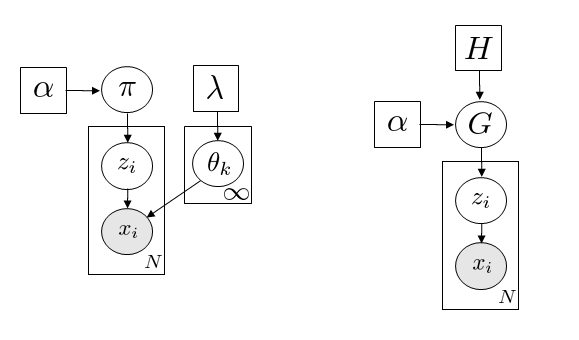
\includegraphics[width=0.6\textwidth, trim={10 10 10 10}]{figures/dpmm_gm.png}
    \caption{DPMM Graphical Model}
    \label{fig:dpmm_gm}
\end{figure}
For each data point $x_i$, there's a corresponding label $z_i$ that assigns the point to one of the clusters with mixture weight $\pi_k$ and parameters $\theta_k = {\mu_k, \Sigma_k}$. The generative model can be written as follows:
\begin{eqnarray}
    p(x_i|z_i=k,\theta) = p(x_i|\theta_k) \\
    p(z_i=k|\pi) = \pi_k \\
    p(\pi|\alpha) = \mathrm{Dir}(\pi|\alpha) \\
    p(\theta_k|\beta) = \mathrm{NIW}(\mu_k,\Sigma_k|m_0,\kappa_0,\nu_0,S_0)
\end{eqnarray}
An equivalent representation of this model can be written as:
\begin{eqnarray}
    G(\theta) = \sum_{k=1}^{\infty}\pi_k \delta_{\theta_k}
\end{eqnarray}
where $\pi \sim \mathrm{Dir}(\alpha_1,...,\alpha_K)$ and $\theta_k \sim H$. Therefore, $G$ is an infinite mixture of cluster functions of delta functions. In practice, we can construct $G$ using a \textit{stick-breaking construction}:
\begin{eqnarray}
    \beta_k \sim \mathrm{Beta}(1,\alpha)\\
    \pi_k = \beta_k \prod_{l=1}^{k-1}(1-\beta_l) = \beta_k(1-\sum_{l=1}^{k-1}\pi_l)
\end{eqnarray}
This is commonly denoted as $\pi \sim \mathrm{GEM}(\alpha)$. The number of generated mixture components increases with $\alpha$. The hyper-parameter $\alpha$ controls the expected number of clusters:
\begin{eqnarray}
    E[K] = \alpha \times \log(1+n/\alpha)\\
    VAR[K] = \alpha \times \log(1+n/\alpha)
\end{eqnarray}
Thus, the number of clusters grows logarithmically with the number of data points and in direct proportion to $\alpha$ as shown in Figure \ref{fig:dpmm_merged1} 
\begin{figure}[thpb]
    \centering
    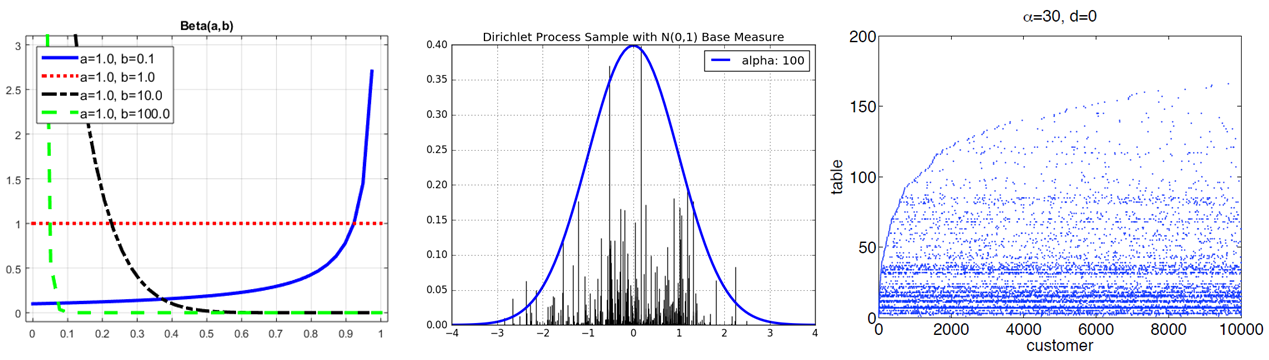
\includegraphics[width=0.9\textwidth, trim={10 10 10 10}]{figures/dp_merged1.png}
    \caption{a) $\mathrm{Beta}(1,\alpha)$ b)DP samples c) DP cluster growth }
    \label{fig:dpmm_merged1}
\end{figure}

\subsection{Fitting a DPMM model}

One way to fit a DPMM is to modify the collapsed Gibbs sampler for a finite mixture model:
\begin{equation}
    p(z_i=k|z_{-i},x,\alpha,\beta) \propto p(z_i=k|z_{-i},\alpha)p(x_i|x_{-i},z_i=k,z_{-i},\beta)
\end{equation}
The first term is given by the Chinese Restaurant Process (CRP):
\begin{equation}
    p(z_i=k|z_{-i},\alpha) = 
    \begin{cases}
        \frac{N_k}{N+\alpha -1} & \text{if } k \text{ is occupied}\\
        \frac{\alpha}{N+\alpha-1} & \text{if } k \text{ is a new cluster}
    \end{cases}
\end{equation}
The second term is the posterior predictive and can be computed as follows:
\begin{equation}
    p(x_i|x_{-i},z_i=k,z_{-i},\beta) = p(x_i|x_{k\setminus i}, \beta) = \frac{p(x_{k}|\beta)}{p(x_{k\setminus i}|\beta)}
\end{equation}
We can compute both the numerator and the denominator above if we can find an expression for the marginal $p(x)$:
\begin{eqnarray}
    p(x) = \int_{\mu} \int_{\Sigma} p(x,\mu,\Sigma) d\mu d\Sigma = \int_{\mu} \int_{\Sigma} p(x|\mu,\Sigma)p(\mu,\Sigma|\beta)d\mu d\Sigma\\
    = (2\pi)^{-ND/2}\frac{Z_{NIW}(D,\kappa_N,\nu_N,S_N)}{Z_{NIW}(D,\kappa_0,\nu_0,S_0)} = \pi^{-ND/2}\frac{\kappa_{0}^{D/2}|S_0|^{\nu_0/2}}{\kappa_{N}^{D/2}|S_N|^{\nu_N/2}}\prod_{i=1}^{D}\frac{\Gamma(\frac{\nu_N+1-i}{2})}{\Gamma(\frac{\nu_0+1-i}{2})}
\end{eqnarray}
Therefore, we can write the second term as follows:
\begin{eqnarray}
    \log p(x_i|x_{k\setminus i}) = z(D,N+1,\kappa_{N+1},\nu_{N+1},S_{Ni}) - z(D,N,\kappa_{N},\nu_N,S_N)\\
    z(D,N,\kappa,\nu,S) = -\frac{ND}{2}\log \pi - \frac{D}{2}\log \kappa - \frac{\nu}{2}\log |S| + \sum_{i=1}^{D}\log \Gamma(\frac{\nu+i-1}{2})
\end{eqnarray}
We can summarize, the collapsed Gibbs sampler for an infinite Gaussian mixture model in Algorithm \ref{alg:dpmm_collapsed}.
\begin{algorithm}
\caption{Collapsed Gibbs for DPMM}
\label{alg:dpmm_collapsed}
\begin{algorithmic}[1]
\STATE Initialize labels $z$ 
\STATE for t = 1,2,...,T do 
\STATE ~~~ for i = 1,2,...,N do 
\STATE ~~~ ~~~ remove $x_i$'s statistics from component $z_i$ 
\STATE ~~~ ~~~ delete empty component
\STATE ~~~ ~~~ for k = 1,2,...,K+1 do
\STATE ~~~ ~~~ ~~~ compute $\log p(z_i=k|z_{-i},x,\alpha,\beta) \sim$
\STATE ~~~ ~~~ ~~~ $\log p(z_i = k|z_{-i},\alpha) + \log p(x_i|x_{k\setminus i},\beta)$
\STATE ~~~ ~~~ sample $z_i = k_{new}$ from $p(z_i=k|z_{-i},x,\alpha,\beta)$
\STATE ~~~ ~~~ create a new cluster if $z_i = K+1$
\STATE ~~~ ~~~ add $x_i$'s statistics to component $z_i = k_{new}$ 
\STATE ~~~ end for
\STATE end for
\end{algorithmic}
\end{algorithm}

Figure \ref{fig:dp_results} shows the clustering results of DPMM collapsed gibbs sampler after 100 iterations on a synthetic dataset of $1K$ points in 2D.
\begin{figure}[thpb]
    \centering
    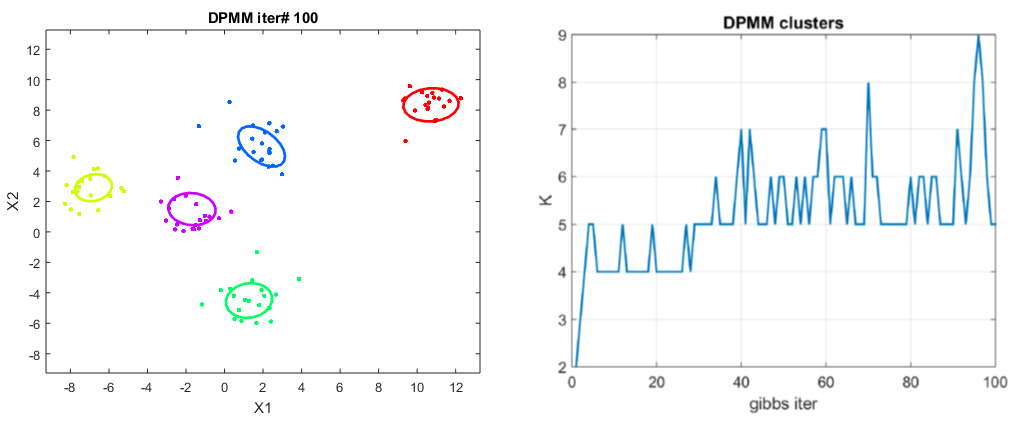
\includegraphics[width=0.8\textwidth, trim={10 10 10 10}]{figures/dp_results.png}
    \caption{DPMM Clustering Results}
    \label{fig:dp_results}
\end{figure}
